% !TeX spellcheck = en_US
% !TeX encoding = utf8
% !TeX program = xelatex
% !BIB program = bibtex

\documentclass[12pt,notes,mathserif]{beamer}
% \documentclass[draft]{beamer}	
\usetheme{Singapore}
% \usetheme{Hannover}
%\usepackage{pgfpages}
%\setbeameroption{show notes on second screen}

\usepackage[british]{babel}
\usepackage{graphicx,hyperref,url}
\usepackage{mmstyles,bm,ulem}

\usepackage{listings}
\usefonttheme[onlymath]{serif}
\usepackage{fontspec}
\usepackage{xeCJK}
% \setCJKfamilyfont{hei}{SimHei}
% \setCJKmainfont[BoldFont=Arial, ItalicFont=Arial]{Arial}
% \pgfdeclareimage[width=\paperwidth,height=\paperheight]{bg}{background}
% \setbeamertemplate{background}{\pgfuseimage{bg}}
%% columns
\newcommand{\begincols}[1]{\begin{column}{#1}}
\newcommand{\stopcols}{\end{column}}
\newcommand{\pp}[2]{\frac{\partial #1}{\partial #2}}
% \usepackage[backend=biber]{biblatex}
% \bibliography{./ref.bib}
%\addbibresource{ref.bib}
\usepackage{indentfirst}
\usepackage{longtable}
\usepackage{float}
\usepackage{rotating}
\usepackage{subfigure}
\usepackage{tabu}
\usepackage{amsmath}
\usepackage{amssymb}
\usepackage{setspace}
\usepackage{amsfonts}
\usepackage{appendix}
\usepackage{listings}
\usepackage{xcolor}
\usepackage{colortbl}
\usepackage{geometry}
% \setCJKfamilyfont{cjkhwxk}{SimSun}
% \newcommand*{\cjkhwxk}{\CJKfamily{cjkhwxk}}
%\newfontfamily{\consolas}{Consolas}
%\newfontfamily{\monaco}{Monaco}
%\setmonofont[Mapping={}]{Consolas}	%英文引号之类的正常显示,相当于设置英文字体
%\setsansfont{Consolas} %设置英文字体 Monaco, Consolas,  Fantasque Sans Mono
% \setmainfont{Times New Roman}
% \newfontfamily{\consolas}{Times New Roman}
% \newfontfamily{\monaco}{Arial}
% \setCJKmainfont{Times New Roman}
%\setmainfont{MONACO.TTF}
%\setsansfont{MONACO.TTF}
\newcommand{\verylarge}{\fontsize{60pt}{\baselineskip}\selectfont}  
\newcommand{\chuhao}{\fontsize{44.9pt}{\baselineskip}\selectfont}  
\newcommand{\xiaochu}{\fontsize{38.5pt}{\baselineskip}\selectfont}  
\newcommand{\yihao}{\fontsize{27.8pt}{\baselineskip}\selectfont}  
\newcommand{\xiaoyi}{\fontsize{25.7pt}{\baselineskip}\selectfont}  
\newcommand{\erhao}{\fontsize{23.5pt}{\baselineskip}\selectfont}  
\newcommand{\xiaoerhao}{\fontsize{19.3pt}{\baselineskip}\selectfont} 
\newcommand{\sihao}{\fontsize{14pt}{\baselineskip}\selectfont}      % 字号设置  
\newcommand{\xiaosihao}{\fontsize{12pt}{\baselineskip}\selectfont}  % 字号设置  
\newcommand{\wuhao}{\fontsize{10.5pt}{\baselineskip}\selectfont}    % 字号设置  
\newcommand{\xiaowuhao}{\fontsize{9pt}{\baselineskip}\selectfont}   % 字号设置  
\newcommand{\liuhao}{\fontsize{7.875pt}{\baselineskip}\selectfont}  % 字号设置  
\newcommand{\qihao}{\fontsize{5.25pt}{\baselineskip}\selectfont}    % 字号设置 

\graphicspath{{./fig/}}

% \setbeamertemplate{footnote}{%
%   \hangpara{2em}{1}%
%   \makebox[2em][l]{\insertfootnotemark}\footnotesize\insertfootnotetext\par%
% }

\definecolor{cred}{rgb}{0.6,0,0}
\definecolor{cgreen}{rgb}{0.25,0.5,0.35}
\definecolor{cpurple}{rgb}{0.5,0,0.35}
\definecolor{cdocblue}{rgb}{0.25,0.35,0.75}
\definecolor{cdark}{rgb}{0.95,1.0,1.0}
\lstset{
	language=R,
	numbers=left,
	numberstyle=\tiny\color{black},
	keywordstyle=\color{cpurple}\consolas,
	commentstyle=\color{cgreen}\consolas,
	stringstyle=\color{cred}\consolas,
	frame=single,
	escapeinside=``,
	xleftmargin=1em,
	xrightmargin=1em, 
	backgroundcolor=\color{cdark},
	aboveskip=1em,
	breaklines=true,
	tabsize=3
} 

\providecommand{\tightlist}{%
	\setlength{\itemsep}{0pt}\setlength{\parskip}{0pt}}

	
\title{Support Vector Machines
vs Logistic Regression}

\author[YingmingLi]{Yingming Li \\ yingming@zju.edu.cn}

\institute[DSERC, ZJU]{Data Science \& Engineering Research Center, ZJU}

\date[\today]{\today}

\begin{document}

\AtBeginSection[]
{
	\begin{frame}
		\frametitle{Outline}
		\tableofcontents[currentsection]
	\end{frame}
}

% \AtBeginSubsection[2-]
% {
%    \begin{frame}
%        \frametitle{Outline}
%        \tableofcontents[currentsection]
%    \end{frame}
% }
\begin{frame}[c]
	\titlepage
	\begin{center}
		Adapted from Prof. Kevin Swersky's slides. 
		
	\end{center}
\end{frame}

\section{}\label{section}

\begin{frame}{Logistic regression}

\begin{center}
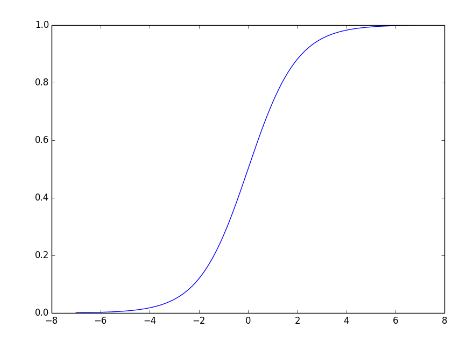
\includegraphics[width=.9\textwidth]{2018-04-15-19-48-36.png}
\end{center}

\end{frame}

\begin{frame}{Logistic regression}

\begin{itemize}
\item
  Assign probability to each outcome \[P(y=1|x)=\sigma(w^{T}x+b)\]
\item
  Train to maximize likelihood
  \[l(w)=-\Sigma_{n=1}^{N}\sigma(w^{T}x_{n}+b)^{y_{n}}(1-\sigma(w^{T}x_{n}+b))^{(1-y_{n})}\]
\item
  Linear decision boundary (with \(y\) being \(0\) or 1)
  \[y=\vone [w^{T}x+b\geq 0]\]
\end{itemize}

\end{frame}

\begin{frame}{Support vector machines}

\begin{center}
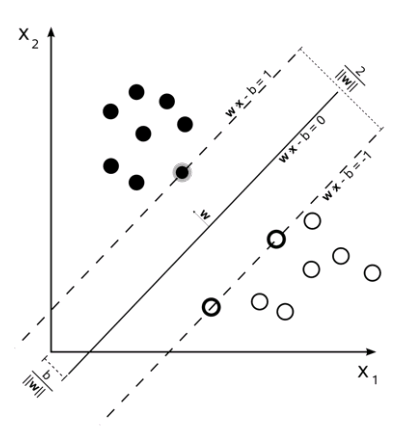
\includegraphics[width=.7\textwidth]{2018-04-15-19-55-03.png}
\end{center}

\end{frame}

\begin{frame}{Support vector machines}

\begin{itemize}
\tightlist
\item
  Enforce a margin of separation \((\)here, \(y\in\{0,1\})\) \[
  (2y_{n}-1)w^{T}x_{n}\geq 1,\ \forall n=1\ldots N
  \]
\item
  Train to find the maximum margin \[
  \min\quad \frac{1}{2}||w||^{2}
  \] \[
  \textrm{s.t.}\quad (2y_{n}-1)(w^{T}x_{n}+b)\geq 1,\ \forall n=1\ldots N
  \]
\item
  Linear decision boundary \[
  \hat{y}=\vone[w^{T}x+b\geq 0]   
  \]
\end{itemize}

\end{frame}

\begin{frame}{Recap}

\begin{itemize}
\item
  Logistic regression focuses on maximizing the probability of the data.
  The farther the data lies from the separating hyperplane (on the
  correct side), the happier LR is.
\item
  An SVM tries to find the separating hyperplane that maximizes the
  distance of the closest points to the margin (the support vectors). If
  a point is not a support vector, it doesn't really matter.
\end{itemize}

\end{frame}

\begin{frame}{A different take}

\begin{itemize}
\item
  Remember, in this example \(y\in\{0,1\}\)
\item
  Another take on the LR decision function uses the probabilities
  instead:
\end{itemize}

\[\hat{y}=\left\{\begin{array}{ll}
1 & \text{if}\ P(y=1|x)\geq P(y=0|x)\\
0 & \text{otherwise}
\end{array}\right.\] \[
P(y=1|x)\propto\exp(w^{T}x+b)
\] \[
P(y=0|x)\propto 1
\]

\end{frame}

\begin{frame}{A different take}

\begin{itemize}
\item
  What if we don't care about getting the right probability, we just
  want to make the right decision?
\item
  We can express this as a constraint on the likelihood ratio, \[
  \frac{P(y=1|x)}{P(y=0|x)}\underline{>}c
  \]
\item
  For some arbitrary constant \(c>1.\)
\end{itemize}

\end{frame}

\begin{frame}{A different take}

\begin{itemize}
\tightlist
\item
  Taking the \(\log\) of both sides, \[
  \log(P(y=1|x))-\log(P(y=0|x))\geq\log(c)
  \]
\item
  and plugging in the definition of \(P,\) \[
  w^{T}x+b-0\underline{>}\log(c)
  \] \[
  \Rightarrow(w^{T}x+b)\underline{>}\log(c)
  \]
\item
  \(c\) is arbitrary, so we pick it to satisfy \(\log(c)=1\) \[
  w^{T}x+b\geq 1
  \]
\end{itemize}

\end{frame}

\begin{frame}{A different take}

\begin{itemize}
\item
  This gives a feasibility problem (specifically the perceptron problem)
  which may not have a unique solution.
\item
  Instead, put a quadratic penalty on the weights to make the solution
  unique: \[
  \min\ \frac{1}{2}||w||^{2}
  \]
  \[\textrm{s.t. }\ (2y_{n}-1)(w^{T}x_{n}+b)\geq 1, \forall n=1\ldots N\]
\item
  This gives us an SVM!
\item
  We derived an SVM by asking LR to make the right \emph{decisions}.
\end{itemize}

\end{frame}

\begin{frame}{The likelihood ratio}

\begin{itemize}
\tightlist
\item
  The key to this derivation is the likelihood ratio, \[
  r=\frac{P(y=N|x)}{P(y=0|x)}
  \] \[
  \qquad=\frac{\exp(w^{T}x+b)}{1}
  \] \[
  \qquad=\exp(w^{T}x+b)
  \]
\item
  We can think of a classifier as assigning some cost to \(r.\)
\item
  Different costs \(=\) different classifiers.
\end{itemize}

\end{frame}

\begin{frame}{LR cost}

\begin{itemize}
\tightlist
\item
  Pick\\

  \begin{align*}
  \textrm{cost}(r)&=\displaystyle \log(1+\frac{1}{r}) \\ 
  &=\log(1+\exp(-(w^{T}x+b)))
  \end{align*}
\item
  This is the LR objective (for a positive example)!
\end{itemize}

\end{frame}

\begin{frame}{SVM with slack variables}

If the data is not linearly separable, we can change the program to: \[
\min\ \frac{1}{2}||w||^{2}+\sum_{n=1}^{N}\xi_{n}
\]
\[\textrm{s.t. }\ (2y_{n}-1)(w^{T}x_{n}+b)\geq 1-\xi_{n}, \forall n=1\ldots N\]
\[
\xi_{n}\geq 0,\ \forall n=1\ldots N
\] Now if a point \(n\) is misclassified, we incur a cost of
\(\xi_{n}\), it's distance to the margin.

\end{frame}

\begin{frame}{SVM with slack variables cost}

\begin{itemize}
\tightlist
\item
  Pick cost

  \begin{align*}
  \textrm{cost}(r) & = \max(0,1-\log(r))\\
  &=\max(0,1-(w^{T}x+b))
  \end{align*}
\end{itemize}

\end{frame}

\begin{frame}{LR cost vs SVM cost}

Plotted in terms of \(r,\)

\begin{center}
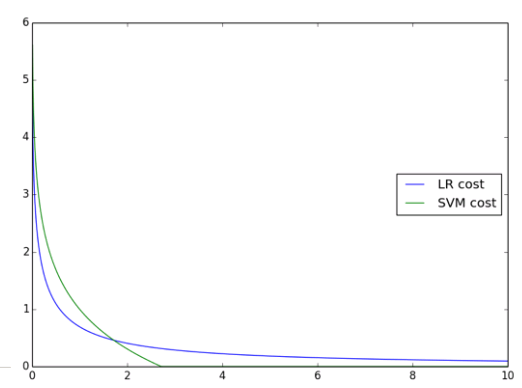
\includegraphics[width=.9\textwidth]{2018-04-15-20-10-15.png}
\end{center}

\end{frame}

\begin{frame}{LR cost vs SVM cost}

Plotted in terms of \(w^{T}x+b,\)

\begin{center}
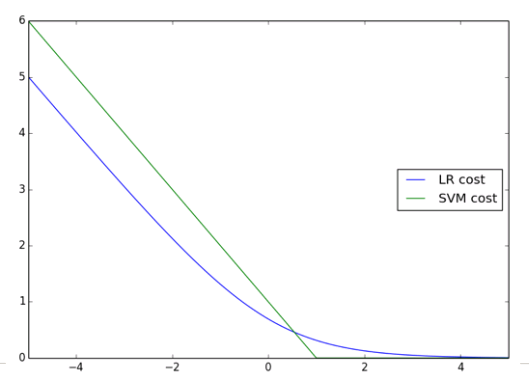
\includegraphics[width=.9\textwidth]{2018-04-15-20-10-37.png}
\end{center}

\end{frame}

\begin{frame}{Exploiting this connection}

\begin{itemize}
\item
  We can now use this connection to derive extensions to each method.
\item
  These might seem obvious (maybe not) and that's usually a good thing.
\item
  The important point though is that they are \emph{principled}, rather
  than just hacks. We can trust that they aren't doing anything crazy.
\end{itemize}

\end{frame}

\begin{frame}{Kernel trick for LR}

\begin{itemize}
\item
  Recall that in it's dual form, we can represent an SVM decision
  boundary as: \[
  w^{T}\phi(x)+b=\sum_{n=1}\alpha_{n}K(x,\ x_{n})=0
  \] where \(\phi(x)\) is an \(\infty\)-dimensional basis expansion of
  \(x.\)
\item
  Plugging this into the LR cost: \[
  \log(1+\exp(-\sum_{n=1}^{N}\alpha_{n}K(x,\ x_{n})))
  \]
\end{itemize}

\end{frame}

\begin{frame}{Multi-class SVMs}

Recall for multi-class LR we have: \[
P(y=i|x)=\frac{\exp(w_{i}^{T}x+b_{i})}{\sum_{k}\exp(w_{k}^{T}x+b_{k})}
\]

\end{frame}

\begin{frame}{Multi-class SVMs}

Suppose instead we just want the decision rule to satisfy: \[
\frac{P(y=i|x)}{P(y=k|x)}\geq c \quad \forall k\neq i
\] Taking logs as before, this gives: \[
w_{i}^{T}x-w_{k}^{T}x\geq 1 \quad \forall k\neq i
\]

\end{frame}

\begin{frame}{Multi-class SVMs}

\begin{itemize}
\tightlist
\item
  This produces the following quadratic program:
\end{itemize}

\(\displaystyle \min \displaystyle \frac{1}{2}||w||^{2}\)
\(\textrm{s.t. }\ (w_{y_{n}}^{T}x_{n}+b_{y_{n}})-(w_{k}^{T}x_{n}+b_{k})\geq 1, \forall n=1\ldots N, \forall k\neq y_{n}\)

\end{frame}

\begin{frame}{Take-home message}

\begin{itemize}
\item
  Logistic regression and support vector machines are closely linked.
\item
  Both can be viewed as taking a probabilistic model and minimizing some
  cost associated with misclassification based on the likelihood ratio.
\item
  This lets us analyze these classifiers in a decision theoretic
  framework.
\item
  It also allows us to extend them in principled ways.
\end{itemize}

\end{frame}

\begin{frame}{Which one to use?}

\begin{itemize}
\item
  As always, depends on your problem.
\item
  LR gives calibrated probabilities that can be interpreted as
  confidence in a decision.
\item
  LR gives us an unconstrained, smooth objective.
\item
  LR can be (straightforwardly) used within Bayesian models.
\item
  SVMs don't penalize examples for which the correct decision is made
  with sufficient confidence. This may be good for generalization.
\item
  SVMs have a nice dual form, giving sparse solutions when using the
  kernel trick (better scalability).
\end{itemize}

\end{frame}

\begin{frame}
	\begin{center}
		\chuhao Thank you!  
	\end{center}
\end{frame}
\end{document}
